\documentclass[12pt,a4paper]{article}
\usepackage{times}
\usepackage[english]{babel}
\usepackage{durhampaper}
\usepackage{harvard}
\usepackage{graphicx}

\citationmode{abbr}
\bibliographystyle{agsm}

\title{AI for Autonomous Agents in Games and Simulations}
\student{James King}
\supervisor{Magnus Bordewich}
\degree{BSc Computer Science}

\date{\today}

\begin{document}

\maketitle

\begin{abstract} {\bf Context:} Designing the core autonomous behaviour for characters in a video game where those characters are expected by the player to perform tasks for themselves poses many interesting challenges. This paper explores the tasks faced when developing a capable and somewhat convincing set of Artificial Intelligence routines within a simulated zombie epidemic real-time strategy game with player allocated goals.
{\bf Aims:} As the game player doesn't have direct control over the characters, but instead can assign tasks, algorithms to allow the characters to plan and implement those tasks in a cooperative and efficient manor will need to be designed. These algorithms must not be computationally expensive to allow for many agents to act in real-time, and also express superficially convincing human-like behaviours.
{\bf Method:} At least two conceptually distinct designs for character behaviour will be designed, and additionally several slight variations of each. These will all be compared in terms of the ability for characters to achieve assigned tasks, avoid threats, and system resource usage. A hybrid between the main designs may be explored if one is not universally better than the other.
{\bf Proposed Solution:} A Subsumptive architecture will initially be explored, followed by a Belief-Desires-Intentions model. Following this, each approach will be adapted to experiment with different character behaviours and strategies including weighting self defence against fleeing, and group formation approaches.
\end{abstract}

\begin{keywords}
AI, BDI, cooperative, multi-agent, subsumptive, task planning, video game
\end{keywords}

\section{Introduction}
\subsection{Context}\noindent
Video game worlds are often populated with Non-Player Characters (or NPCS), the behaviour of which can make or break the game. A great deal of effort is required when designing the routines used by these characters if they are to satisfy some major requirements; they should behave with approximate rationality, they should provide an appropriate challenge for the player, and if the characters represent humans (or at least animals) they should act in a believable way. For Real-Time Strategy (or RTS) games the difficulty is further accentuated by the necessity of the game to support perhaps hundreds or even thousands of these characters in an environment simultaneously. This combines the previous three requirements with a fourth: efficiency. Designing solutions for the first three key requirements is often more of a creative task rather than a purely methodical one, and entails an element of subjectivity. The fourth requirement is easier to test, but the difficulty in maintaining a minimum performance quality heavily depends on the complexity of the solutions for the first three goals.

\subsection{Problem Domain}\noindent
This project aims to explore possible implementations of an NPC behaviour system designed to realise the central gameplay of a work-in-progress RTS game. The components of the game that existed prior to the beginning of this project form a zombie epidemic simulation. A city environment is procedurally generated, producing buildings separated by streets. When this process is complete, a number of human characters are dispersed around the environment, a fraction of which initialise as a zombie. The simulation then begins, with the zombies navigating towards the nearest visible human, and humans attempting to run away from danger if any is present (and otherwise just wandering randomly). If a zombie catches up to a human it may attack it, reducing a stored health value for that human and infecting that human with some probability. If a human loses all their health and is infected, they become a zombie too.

The conflict is clearly one-sided, not least because the zombies are smarter than the humans. The humans have little regard for their surroundings other than the locations of visible enemies, and so often run directly into the inner corners of walls. This would obviously not a sufficient behaviour; looking at the core requirements for a decent NPC it fails at being rational, at providing an appropriate challenge (the humans don't stand a chance), and they certainly don't act like humans. Their only redeeming quality is that their simple AI isn't too computationally expensive, so thousands of them can be supported simultaneously.

\subsection{Project Aims}\noindent
At the very least the artificial intelligence routines explored in this project should improve each human agent's survival ability. This may mean attempting to escape when cornered, deciding when it is rational to attack in self defence, and implementing strategies to hide from danger. Later on in the project a player will be able to assign actions for the humans to complete, such as instructing a group to navigate to a specific location, or to construct barricades out of material found in buildings. These commands may conflict with an agent's necessity for self preservation, so the processes developed should intelligently decide when it is rational to belay an order.

On the topic of player-specified tasks, an efficient path finding technique will need to be implemented that balances time required to processes with optimality of the path found. This algorithm will be essential for when agents are directed to a specified location by the player, but also useful for attempting to navigate when performing other tasks or to detect if a path exists to bypass some barricades (establishing whether they are safe). Some tasks may not be assigned to a specific agent but will rather be goals to be achieved by the collective group. For example, the player will be able to instruct that a barricade should be built in a specific location. In this instance the human agents should automatically distribute sub-tasks between themselves in order to achieve the common goal efficiently.

The two core approaches to be compared are a Subsumptive architecture and a Belief-Desires-Intentions model. A subsumptive architecture features a stack of behaviour layers where each may in turn choose to either act or subsume control to the next layer, starting with the top of the stack. The first layer in the sequence to specify an action is heeded, and the rest are ignored. This design usually relies on complex behaviour emerging from complimentary layers. A Belief-Desires-Intentions model is a radically different approach, where each agent records a formal representation of the world from which a set of attainable goals are found, a subset of which is acted upon according to estimated rationality.

\subsection{Deliverables}\noindent
These following core elements will be created before the end of the project.

\begin{enumerate}
  \deliverable{Expanded Core Game}
  {The central mechanics that the AI system will interact with must be implemented. These include the creation of game objects that represent a resource to be used when building barricades, the system to support the construction of the barricades themselves, and an expanded user interface which allows a player to select groups of agents and assign tasks. Additionally facilities to be used by the two proposed architectures should be provided, such as a path-finding implementation.}

  \deliverable{Subsumptive Prototype}
  {An agent design using a subsumptive architecture will be developed, implementing the core requirements of the human NPCs. This prototype will be constructed by breaking up the human's functionality into a stack of behaviours, from which a successful strategy is designed to emerge. Relies on deliverable 1.}

  \deliverable{BDI Prototype}
  {A distinct agent design using a BDI architecture will also be developed, meeting the same requirements as the subsumptive approach. This prototype will use a personal abstracted representation of the environment for each human agent, from which a set of achievable goals are found using a goal evaluation algorithm. These goals are then further reduced into a set that is calculated to yield the most utility, and are simultaneously possible. Relies on deliverable 1.}

  \deliverable{Analysis \& Final Report}
  {Both completed prototypes will be analysed and compared in terms of agent survival rate (without player intervention), efficiency at which goals specified by a player are achieved, prevalence of unnatural behaviour, and system resource usage. The results of this comparison will be compiled into a report, along with the identification of the prototype that is most suited for the problem and an explanation for why that prototype was chosen. The report will also cover possible areas of additional research exposed by this project. Relies on deliverables 2 and 3.}
\end{enumerate}

\section{Design}
\subsection{Requirements}\noindent
The main deliverable can be broken down into a set of core functional and non-functional requirements, each with a relative priority rating. These requirements have been categorised into the Core Requirements that the existing game will be extended to fulfil, and the AI Requirements that the two agent design prototypes must independently satisfy. Functional requirements are prefixed with `FR', while non-functional requirements are prefixed with `NFR'.

\subsubsection{Core Requirements}
\begin{requirements}
\requirement{FR}{Med}{% FR 1.1
  The number of initial humans, zombies, and the world size must be configurable.
}

\requirement{FR}{High}{% FR 1.2
  NPCs must be able to navigate between any two positions in the game environment if a path exists.
}

\requirement{FR}{Med}{% FR 1.3
  Game objects representing a resource used when constructing barricades must exist within the game environment.
}

\requirement{FR}{High}{% FR 1.4
  NPCs must have the ability to construct barricades, ideally using resource objects (FR 1.3).
}

\requirement{FR}{Med}{% FR 1.5
  A player must be able to select a group of human agents through the user interface.
}

\requirement{FR}{Med}{% FR 1.6
  A player must be able to instruct selected agents (FR 1.5) to move to a chosen location.
}

\requirement{FR}{Med}{% FR 1.7
  A player must be able to instruct selected agents (FR 1.5) to block off a specified area with a barricade.
}

\requirement{FR}{High}{% FR 1.8
  An analysis of the scalability of the game environment must be produced, exploring how the environment size and number of agents affects performance.
}

\requirement{NFR}{Med}{% NFR 1.9
  The simulation must be able to maintain an average frame time of at most 16.67ms with a world size of 128x128 tiles and 250 active agents.
}

\requirement{NFR}{Low}{% NFR 1.10
  Moving objects within the game environment must not pass through solid geometry outside of exceptional circumstances that would not occur during standard gameplay.
}

\requirement{NFR}{Low}{% NFR 1.11
  NPCs must demonstrate an ability to recognise whether a specified object is visible, and not react to things they should not be aware of.
}
\end{requirements}

\subsubsection{AI Requirements}
\begin{requirements}
\requirement{FR}{High}{% FR 2.1
  Human agents must exhibit a strategy for avoiding or eliminating nearby visible threats.
}

\requirement{FR}{High}{% FR 2.2
  Human agents must be able to navigate to a position as instructed by a player (using FR 1.8), unless this conflicts with FR 2.1.
}

\requirement{FR}{Med}{% FR 2.3
  Human agents must possess the ability to autonomously construct barricades to block off areas without player direction.
}

\requirement{FR}{High}{% FR 2.4
  Human agents must possess the ability to construct barricades to block off areas specified by a player (using FR 1.9).
}

\requirement{FR}{High}{% FR 2.5
  An analysis of the survival rate and efficiency at which player assigned tasks are achieved must be produced.
}

\requirement{NFR}{Low}{% NFR 2.6
  Agents should exhibit erratic or unnatural behaviour only rarely, if at all.
}
\end{requirements}

\subsection{Implementation}\noindent
Several key elements of this project require a non-trivial amount of planning and design, the details of which will be described in this section.

\subsubsection{Path Finding \& Navigation}

\begin{figure}[h]
\centering
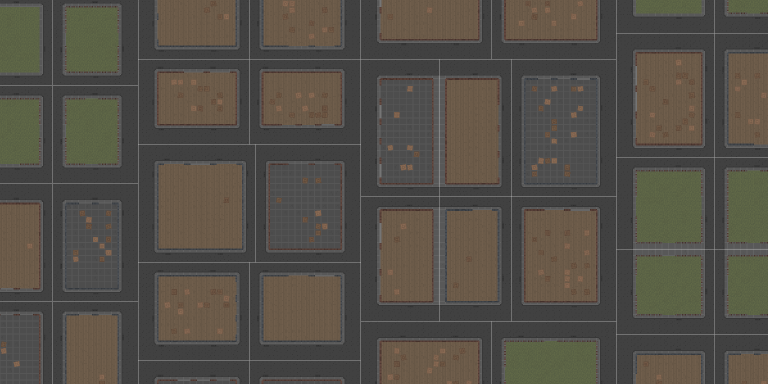
\includegraphics[width=0.9\textwidth]{blocks}
\caption{A diagram to show the structure of a procedurally generated city environment, featuring blocks of buildings separated by roads. Each block is bounded by a white rectangle.}
\end{figure}

\subsubsection{Vision \& Collision Testing}

\subsubsection{Subsumptive Prototype}

\subsubsection{BDI Prototype}

\subsubsection{Analysis Strategy}

\bibliography{report}


\end{document}
